\documentclass[14pt]{beamer}
\title[JPL:Java:02]{JPL :: Strings}
\author[TS]{TalentSprint}
\institute[L\&D]{Licensed To Skill}
\date{Version 1.0.4}
\usefonttheme{serif}
\usecolortheme{orchid}
\usepackage{bookman}
\usepackage{hyperref}
\usepackage[T1]{fontenc}
\usepackage{graphicx}
\usepackage{listings}
\graphicspath{{../../Images/}}
\beamertemplateballitem
\usebackgroundtemplate{
\includegraphics[width=\paperwidth]{TS-Logo.jpg}}
\lstset{language=Java,numbers=left, numberstyle=\tiny, basicstyle=\footnotesize, numbersep=10pt, showstringspaces=false, breaklines=true,keepspaces=true, columns=flexible}
\begin{document}

\begin{frame}
  \titlepage
\end{frame}

\begin{frame}{Learning Objectives}
The content in this presentation is aimed at teaching  learners to:
\begin{itemize}
\item write programs that use and manipulate strings in Java.
\end{itemize}
\end{frame}

\begin{frame}{Strings}
\begin{figure}[H]
\begin{center}
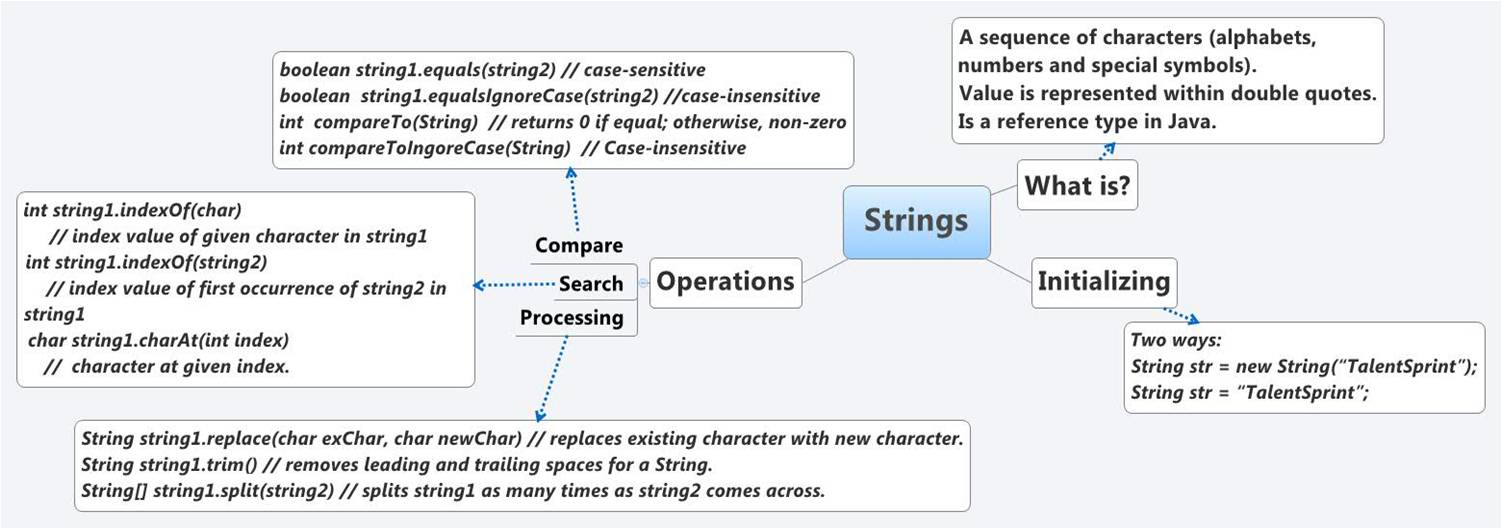
\includegraphics[scale=.4]{strings.jpg}
\end{center}
\end{figure}
\end{frame}

\begin{frame}[fragile]{Strings}
Let us recollect the Java program that adds numbers.
\begin{lstlisting}[numbers=none]
public class SumExample2 {
    public static void main(String[] args) {
        int next, sumSoFar;
        next = Integer.parseInt(args[0]);
        sumSoFar = next;
        next = Integer.parseInt(args[1]);
        sumSoFar += next;
        next = Integer.parseInt(args[2]);
        sumSoFar += next;
        System.out.println("Sum: " + sumSoFar);
    }
}
\end{lstlisting}
\end{frame}

\begin{frame}{Strings}
What is the meaning of \textbf{String[ ]} args in the main method?
\begin{itemize}
\item It is to specify that the parameters of the main method are an array of strings referred to by a variable name args.
\item A sequence of characters each of which can be an alphabet, number or a special symbol.
\item String is a reference type in Java.
\item The value of a String must be within double quotes (" ") e.g.  "Blake"
\end{itemize}
\end{frame}

\begin{frame}[fragile]{Strings}
\textbf{Creating Strings}

Like any other type of variable, a String variable is declared as follows.
\begin{lstlisting}[numbers=none]
String variable_name;
e.g. String name;
Then, a value is assigned as follows.
name = "TalentSprint"; OR
name = new String("TalentSprint"); 
Declaration and assignment can be in one statement. E.g.  
String name = new String("TalentSprint"); OR
String name = "TalentSprint";
\end{lstlisting}
\end{frame}

\begin{frame}[fragile]{Strings}
String Comparison

Strings can not be compared using relational operators such as $<$, $>$, == etc
In stead, an equals() method is used which returns true in case both are equal and false otherwise.
\begin{block}{Example}
\begin{lstlisting}[numbers=none]
String name1 = "James";
String name2 = "adam";
System.out.print(name1.equals(name2));
\end{lstlisting}
\end{block}
\end{frame}

\begin{frame}{Strings}
Methods for String Comparison
\begin{description}
\item [boolean equals(String)] For Case-sensitive comparison
\item [boolean  equalsIgnoreCase(String)] Case-insensitive comparison
\item [int  compareTo(String)] Case-sensitive comparison; Return value of zero means equality, otherwise, inequality
\item [int compareToIngoreCase(String)] Case-insensitive comparison
\end{description}
\end{frame}

\begin{frame}{Strings}
Other operations on Strings
\begin{description}
\item [String toUpperCase(String] Converts lower-case to upper-case
\item [String toLowerCase(String)] Converts upper-case to lower-case
\item [char charAt(int index)] Returns character at given index
\item [char[] toCharArray(String)] Returns character array for given String
\item [int length()] Returns No. Of characters in a String
\end{description}
\end{frame}

\begin{frame}{Strings}
Other operations on Strings
\begin{description}
\item [int indexOf(char)] Returns index value of given character in a String
\item [String replace(char exChar, char newChar)] Replaces existing character with new character
\item [String trim()] Removes leading and trailing spaces for a String
\item [String[] split(String)] Splits the String as many times as given String i.e. parameter comes across and returns parts as a String array.
\end{description}
\end{frame}

\begin{frame}{Strings}
Other operations on Strings
\begin{description}
\item [String substring(int start\_Index, int end\_Index))] Returns sub-string as per given index range
\item [String concat(String)] Joins two strings and returns it
\item [boolean startsWith(String prefix)] Returns true if String starts with given prefix
\item [boolean endsWith(String suffix)] Returns true if String ends with given suffix
\end{description}
\end{frame}

\begin{frame}{Strings}
\small
\begin{enumerate}
\item Write a function that removes all occurrences of vowels in a given string and returns the string without vowels.

\item Write a function which returns the count of number of times the given character exists in a string.

\end{enumerate}
\end{frame}

\begin{frame}{Strings}
\begin{enumerate}
\setcounter{enumi}{2}
\item Write a program which displays the following output.
for a given input : 1,2,3,4,5-8,9,10,11-15,16-25
Output  : 1,2,3,4,5,6,7,8,9,10,11,12,13,14,15,16,17,18,19,20,21,22,23,24,25

\item Two words are called anagrams if they have same letters and each letter occurs same no of times e.g. silent listen	

Write a method which accepts two strings and returns true if they are anagrams else return false.

\end{enumerate}
\end{frame}

\begin{frame}{Strings}
\begin{figure}[H]
 \begin{center}
   
\includegraphics[scale=.3]{qa.png}   
 \end{center}
  \end{figure}
\end{frame}

\end{document}
